\documentclass[12pt]{article}
\usepackage{../../includes/lecture_notes}
\usepackage{../../includes/math}

\newcommand{\answer}[1]{{\color{blue_winged_teal}\textbf{Answer:} #1}}
\newcommand{\pts}[1]{{\color{zinc500}(#1 pts)}}

\begin{document}
\begin{center}
  {\Huge\bf Midterm - Spring 2025}

  \smallskip
  {\large\it ECON 5753 — University of Arkansas}
\end{center}

\medskip
\begin{enumerate}
  \item \pts{10} Say a researcher wants to model the conditional expectation of wages given gender, college degree, and age. The author includes a linear function of age, an indicator for having a college degree, and an indicator for being a female. Suggest a few (2 or 3) additional terms they could include in their model and give a reason why each term might be good to add.

  \answer{
    Examples include:
    \begin{enumerate}
      \item 5-year bins for age: This could be useful if the relationship between age and wages is non-linear.

      \item Interaction between age and college: allow the impact of college to change with age, e.g. wages grow faster for college workers.

      \item Age interacted with gender: model wage-growth separately for male and female workers.
    \end{enumerate}
  }

  \bigskip
  \item \pts{20} Say we have a survey of Americans (like the Current Population Survey). We run a \emph{linear regression} with having gone to college (taking values $0$ and $1$) on indicators for each race (White, Hispanic, Black, Native, and Asian/Pacific Islander). Here are the results:
  \begin{codeblock}[{}]
OLS estimation, Dep. Var.: has_college_experience
Observations: 226,666
Standard-errors: Heteroskedasticity-robust
                                 Estimate Std. Error  t value  Pr(>|t|)
(Intercept)                      0.716339   0.001187 603.5694 < 2.2e-16 ***
race::Asian or Pacific Islander  0.066815   0.003442  19.4098 < 2.2e-16 ***
race::Black                     -0.088041   0.003242 -27.1584 < 2.2e-16 ***
race::Hispanic                  -0.178127   0.002816 -63.2493 < 2.2e-16 ***
race::Native                    -0.167055   0.010281 -16.2492 < 2.2e-16 ***
---
Signif. codes:  0 '***' 0.001 '**' 0.01 '*' 0.05 '.' 0.1 ' ' 1
  \end{codeblock}

  \begin{enumerate}
    \item \pts{5} Interpret the coefficient on the Hispanic indicator. Comment on its statistical significance.

    \answer{
      The coefficient on the Hispanic indicator is -0.178. Compared to White respondents, Hispanic respondens have a 17.8\% lower probability of having attended college. This coefficient is statistically significant at the 1\% level.
    }

    \item \pts{5} We discussed in class concern about linear probablity model predicting fitted probabilities $\hat{\mathbb{P}}( Y_i = 1 \ | \ W_i = w )$ outside of $[0, 1]$. Does that problem come up in this model? Why or why not?

    \answer{
      This problem does not come up since the only explanatory variables are indicators.
    }

    \item \pts{10} What is the estimated difference in rates of having attended college between Hispanic and Native Americans. What would be a simple way to modify this regression to test significance of the difference?

    \answer{
      The differences is -0.178 - (-0.167) = -0.011. This means that Hispanic respondents have a 1.1\% lower probability of having attended college than Native Americans.
      To test the significance of this difference, we could modify our regression to use Hispanic as the reference group.
      Then a test of the Native coefficient would be a test of the difference between the two groups.
    }
  \end{enumerate}

  \item \pts{20} You are analyzing a dataset of high-school basketball players. You have data on their physical attributes, their position played, and basic stats from their senior year.
  \begin{enumerate}
    \item \pts{10} To flexibly model the relationship between points scored and height, you run a model with a 3rd-order polynomial. What concerns might you have with predicting the points scored for a high-school player who is 7'0''.

    \answer{
      Since polynomials shoot off to infinity, we run the risk when predicting for a player that is 7'0''.
      This risk is particularly large since so few players are that tall in our dataset.
    }

    \item \pts{10} Say you want to let the relationship between height and points scored vary by position. Describe the regression you could run that would estimate different slopes by position, i.e. what terms would you include in your model?

    \answer{
      We could run a regression with the following terms:
      \begin{enumerate}
        \item Height
        \item Position indicators
        \item Height interacted with position indicators
      \end{enumerate}
      This would allow us to estimate different slopes for each position.
    }
  \end{enumerate}

  \bigskip
  \item \pts{15} A study analyzed a survey dataset of Americans aged 40-60. The surveys asked them how many drinks they have per week (options were 0, 1-3, 4-6, 7+) and health outcomes (e.g. an indicator for having cardiovascular problems).
  The study found that the compared to 0 drinks, the probability of having cardiovascular problems was 1.5\% lower for people who drank 1-3 drinks per week.
  \begin{enumerate}
    \item \pts{5} Explain what regression the researchers might have run to estimate this.

    \answer{
      The researchers probably ran a regression of health oucomes on indicators for the number of drinks per week they report consuming.
      The reference category woudl be 0 drinks, and they report the coefficient on $\one{\text{1-3 drinks per week}}$.
    }


    \item \pts{10} Why might we be hesitant to not call this evidence the ``causal'' effect of having more drinks?

    \answer{
      When comparing across individuals with different drinking habits, we might be comparing people with different health habits, different social lives, and different socio-economic statuses.
      These other factors could be driving differences in health outcomes.
    }
  \end{enumerate}


  \bigskip
  \item \pts{10} Two classmates are competing to find the best model to predict the winners of NFL games. Both train some kind of logistic regression model using a bunch of different variables with data on the past 3 seasons of games. They compare whose model performs better on their training sample and use the model that performs best. Why might this be a bad idea?

  \answer{
    This is a bad idea because they are using the same data to train and to evaluate their model.
    They could be overfitting their model to the training data, which would make it perform worse on new data.
  }

  \bigskip
  \item \pts{25} Figure \ref{fig:wage_vs_age} presents sample averages of a worker's income for each age (points).
  Additionally, the line presents fitted values from a regression of income on age and age$^2$.
  The regression results are shown below the figure. Answer the following questions:

  \begin{enumerate}
    \item \pts{5} True/False: the sample average for each bin gives an \emph{exact} estimate of the CEF.

    \answer{
      True. The sample average is an unbiased estimator of the CEF.
    }

    \item \pts{5} Predict someone's wage when they are 40 years old. Show your math if you do not have a calculator.

    \answer{
      We can use the regression to predict the wage for a 40-year-old.
      $$
        \hat{y} = -60919.4890 + 5081.4608 \cdot 40 - 49.2057 \cdot 40^2
      $$
      This gives us $\hat{y} = 63,609.82$ or about \$64,000.
    }

    \item \pts{10} What would be the change in wage predicted going from 30 to 31 years old? Show your math if you do not have a calculator.

    \answer{
      The marginal effect is given by
      $$
        5081.4608 + 2 * (-49.2057) * 30 = 2,129.12
      $$

      In words, we predict an increase of \$2,129 in wages going from 30 to 31 years old.
    }

    \item \pts{5} Can you reject a linear relationship between age and income? Why or why not?

    \answer{
      We can reject a linear relationship as teh coefficient on $\text{age}^2$ is statistically significant.
    }
  \end{enumerate}

  \begin{figure}
    \caption{Sample average of wages for each age and a quadratic fit}
    \label{fig:wage_vs_age}
    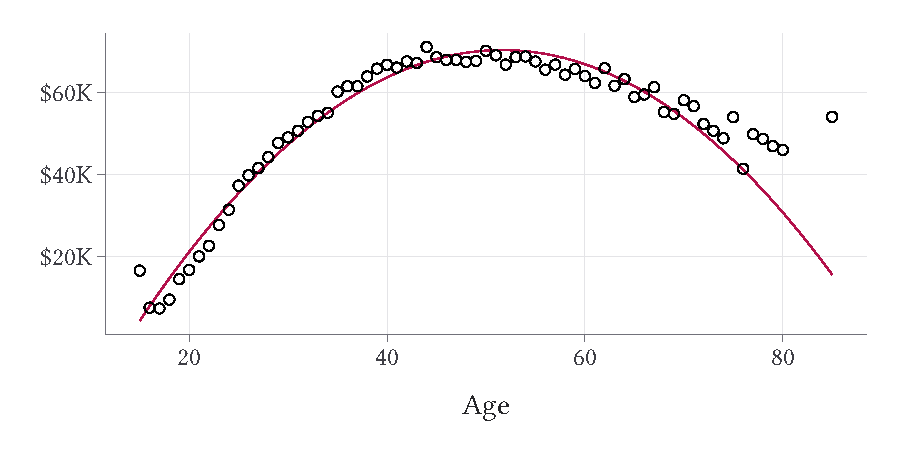
\includegraphics[width = \linewidth]{figures/plot_wage_age.pdf}
  \end{figure}

  \bigskip
  \begin{codeblock}[{}]
OLS estimation, Dep. Var.: incwage
Observations: 226,666
Standard-errors: Heteroskedasticity-robust
                Estimate  Std. Error  t value  Pr(>|t|)
(Intercept) -60919.4890 1005.711304 -60.5735 < 2.2e-16 ***
age           5081.4608   54.379442  93.4445 < 2.2e-16 ***
I(age^2)       -49.2057    0.652094 -75.4579 < 2.2e-16 ***
---
Signif. codes:  0 '***' 0.001 '**' 0.01 '*' 0.05 '.' 0.1 ' ' 1
  \end{codeblock}


\end{enumerate}

\end{document}
